\section{SVN 学习笔记}
\subsection{使用externals属性}
使用情景: 当在svn中多个目录同时引用同一个文件夹的文件,或者多个svn同时引用另外一个svn的内容,当被引用的内容需要修改时,需要去到每个文件夹修改,不方便,在svn中可以采用在引用的文件夹里面增加externals属性,引用该文件夹,设置步骤如下:
\begin{itemize}
\item 在需要引用的svn文件夹,右键,进入属性设置
\begin{figure}[H]
\centering
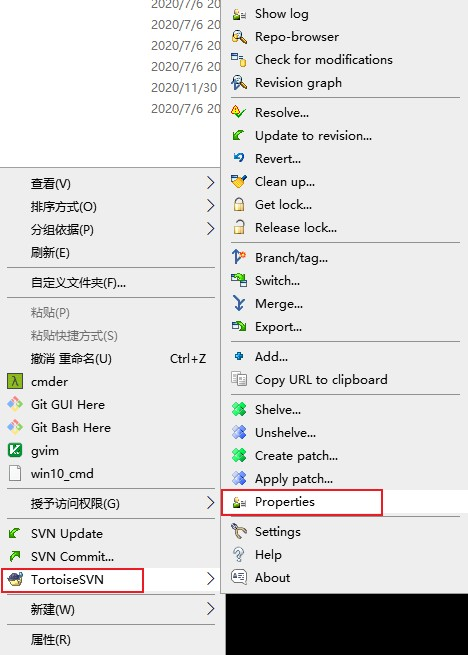
\includegraphics[height=8cm]{svn_externals_1.jpg}
\caption{进入svn属性设置}
\end{figure}

\item 在属性设置界面点击\emphasizebox{New->Externals}
\begin{figure}[H]
\centering
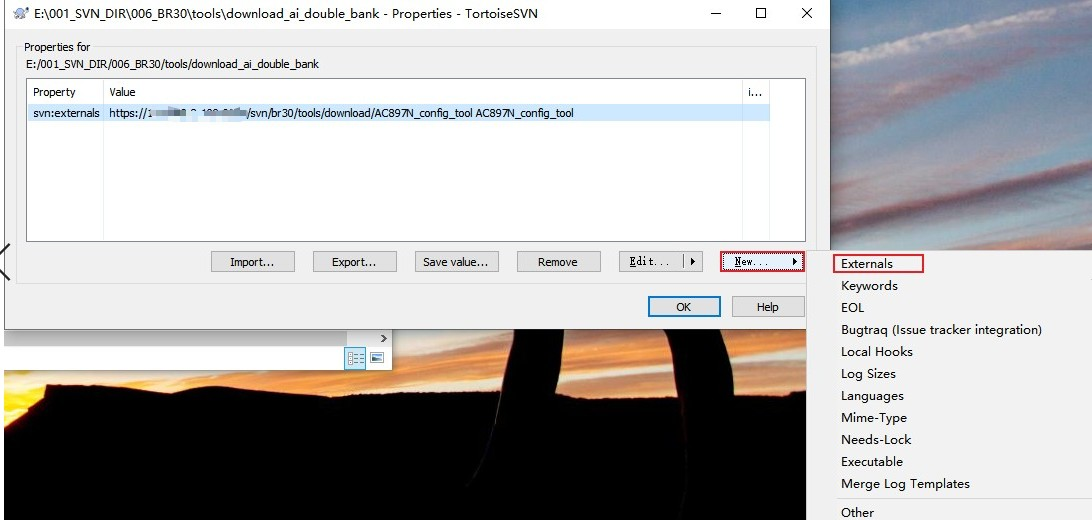
\includegraphics[height=8cm]{svn_externals_2.jpg}
\caption{点击New->Externals}
\end{figure}

\item 进入Externals界面,点击\emphasizebox{New}
\begin{figure}[H]
\centering
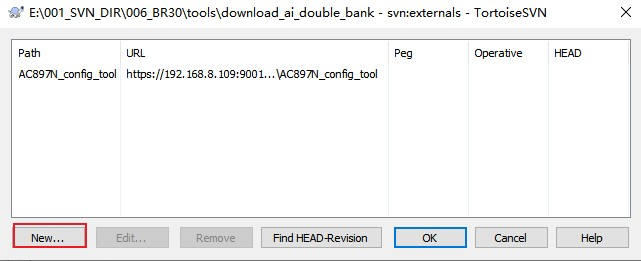
\includegraphics[height=4cm]{svn_externals_3.jpg}
\caption{点击New}
\end{figure}

\item 配置\emphasizebox{Local path}和\emphasizebox{path}
\begin{figure}[H]
\centering
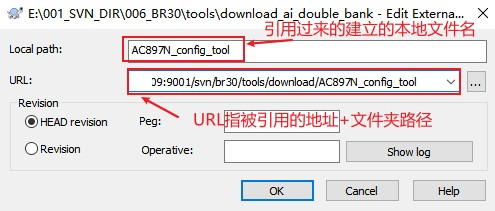
\includegraphics[height=4cm]{svn_externals_4.jpg}
\caption{配置引用信息}
\end{figure}
配置完后点击\emphasizebox{OK}

\item 配置完后,可以看到文件夹属性增加了一项\emphasizebox{svn externals}
\begin{figure}[H]
\centering
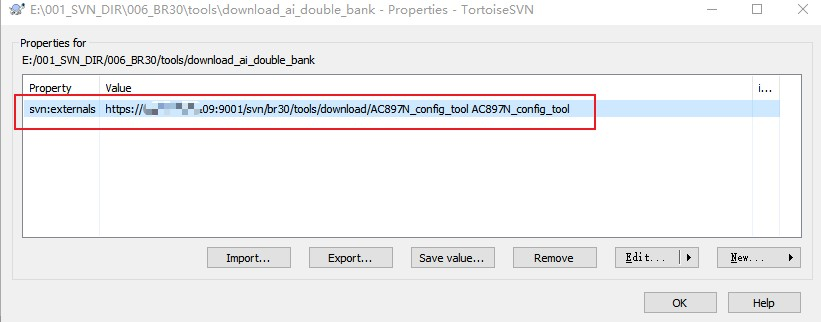
\includegraphics[height=4cm]{svn_externals_5.jpg}
\caption{svn externals信息}
\end{figure}


\item 点击\emphasizebox{svn update}可以把引用的内容拉取过来
\begin{figure}[H]
\centering
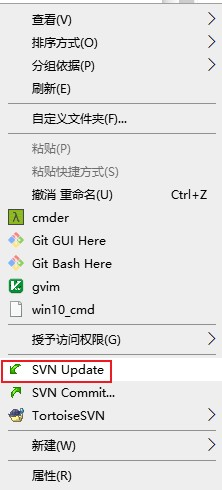
\includegraphics[height=8cm]{svn_externals_6.jpg}
\caption{svn update拉取引用的内容}
\end{figure}

\item 点击\emphasizebox{svn commit}把文件夹增加的属性上传
\begin{figure}[H]
\centering
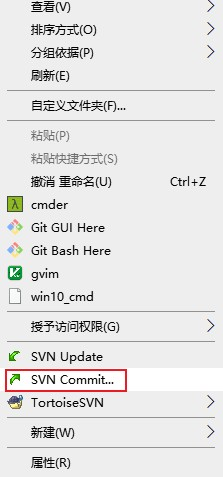
\includegraphics[height=8cm]{svn_externals_7.jpg}
\caption{svn commit上传增加的属性}
\end{figure}

\end{itemize}

至此,svn externals属性增加完成,有如下特性:
\begin{itemize}
\item 修改被引用的内容上传,相应引用的文件夹会同步被修改到;
\item 修改任一文件夹的内容上传,被引用的文件夹也会被修改到;
\item 只有上传之后,再更新引用的文件夹里面的内容才会更新,引用的文件夹内容同步的是远程服务器的内容;
\end{itemize}

\subsection{Linux svn命令行忽略某些文件跟踪}
修改配置文件,路径:
\begin{commandbox}
vim ~/.subversion/config
\end{commandbox}
添加配置项:
\begin{messagebox}
global-ignores = *.o *.lo *.d *.la *.al .libs *.so *.so.[0-9]* *.a *.bin *.pyc *.pyo __pycache__ cscope.out tags filenametags *.bc symbol.txt *resolution.txt *.format_orig
\end{messagebox}

\subsection{Linux svn命令行添加diff工具关联}
修改配置文件,路径:
\begin{commandbox}
vim ~/.subversion/config
\end{commandbox}
添加配置项:
\begin{messagebox}
diff-cmd = meld
\end{messagebox}
